\documentclass{article}
\usepackage{amsmath}
\usepackage{mathtools}
\usepackage{gensymb}
\usepackage[a4paper,inner=1.5cm,outer=1.5cm,top=2cm,bottom=0.5cm]{geometry} 
\usepackage{xcolor}                    
\usepackage{tikz}                           
\usepackage{multicol}
\usepackage{pgfplots}
\usetikzlibrary{calc}
\usetikzlibrary{intersections}
\usetikzlibrary{intersections,calc,angles,quotes}
\usetikzlibrary{shapes,arrows,positioning,decorations.pathreplacing,calc}
\usetikzlibrary{calc,angles,positioning,intersections,quotes,decorations.markings}
\usepackage{tkz-euclide}
\usetikzlibrary{backgrounds}
\usetikzlibrary{calc,through}
\usetikzlibrary{angles}
\usetikzlibrary{fadings}
\usetikzlibrary{shapes.geometric}
\usetikzlibrary{shapes.symbols}
\usepackage{draftwatermark}
\usepackage{mathptmx}

\SetWatermarkText{\textcolor{black!30}{Mathema Shukur}}
\SetWatermarkFontSize{2 cm}
\usepackage[utf8]{inputenc}
\usepackage{fontspec}

\setmainfont{[Kalpurush.ttf]}
\newfontface{\en}{[Arial.ttf]} %%this is optional, if you want to use a secondary font. Any english font is supported
\newlength\Radius
\setlength\Radius{4cm}
\begin{document} 
	\Large
	\textcolor{red}{Welcome To} 
	\\
	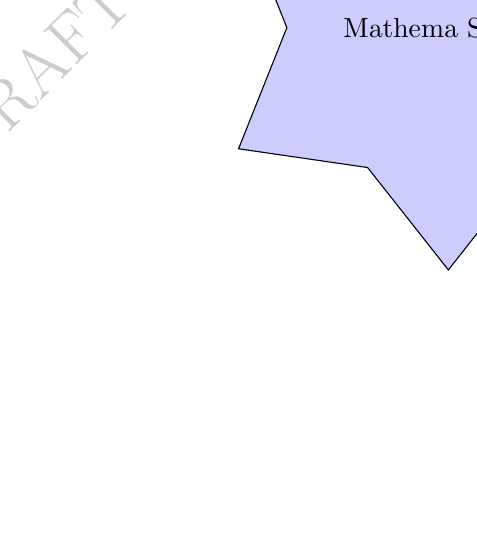
\begin{tikzpicture}
		\tikz \node [fill=blue!20,star,star points=6,draw] {Mathema Shukur };
	\end{tikzpicture}
	\\
	যাদের জন্যে প্রযোজ্যঃ  	\textcolor{magenta}{একাদশ ও দ্বাদশ শ্রেণীর শিক্ষার্থী} \\
	বিষয়ঃ \textcolor{magenta}{উচ্চতর গণিত ১ম পত্র} \\
	অধ্যায়ঃ \textcolor{magenta}{৩-সরলরেখা}\\ 
	Subtopicঃ  \textcolor{magenta}{ সরলরেখার বিভিন্ন আকারের সমীকরণ নির্ণয় করা  }\\
	\\
\textcolor{blue}{(1)	ঢাল বিন্দু আকার Point slope form}\\
\\
$(y-y_1)=m(x-x_1)$\\
\\
 \textcolor{red} {(2)  দুই বিন্দু আকার 	Two point form}\\
 \\
 	$y-y_1=\left(\frac{y_1-y_2}{x_1-x_2}\right)(x-x_1)$\\
 	\\
 \textcolor{green}{ (3) ঢাল খণ্ডন আকার 	Slope intercept form}\\
 \\
 $y=mx+c$\\
 \\
\textcolor{cyan}{ (4) দ্বি খণ্ডন আকার  Two	Intercept form}\\
\\
$\frac{x}{a}+\frac{y}{b}=1$\\
	\\
	রাজশাহী বোর্ড-২০২১\\
	$(2,-3)$ বিন্দুগামী এবং $2$ ঢাল বিশিষ্ট সরলরেখার সমীকরণ নির্ণয় কর \\
	$(x_1,y_1)=(2,-3),\qquad m=2$\\
	\begin{align*}
		(y-y_1)&=m(x-x_1)\\
		\\
		y-(-3)&=2(x-2)\\
		\\
		y+3&=2x-4\\
		\\
		2x-y-7&=0		
	\end{align*}
	\\
		\begin{tikzpicture}[transform shape,scale=1]
		\draw [-latex,thick](-2,0) -- (6,0) node[right] {$x$} coordinate(x axis);
		\draw [-latex,thick](0,-10) -- (0,4) node[above] {$y$} coordinate(y axis);
		\fill[black] (0,0) circle (1 mm);
			\fill[magenta] (2,-3) circle (1 mm);
		\node at (0.3,-0.3) {$\textcolor{purple}{O}$};	
		\node at (3,-3) {$\textcolor{magenta}{(2,-3)}$};	
			\draw[very thick,magenta] (5,3)--(-1,-9);	
	\end{tikzpicture}\\
\\
	সিলেট বোর্ড-২০২১\\
	$(6,-2)$ বিন্দুগামী এবং  $x-$ অক্ষের ধনাত্মক দিকের সাথে  $60\degree$ কোণ উৎপন্ন করে এরুপ সরলরেখার সমীকরণ নির্ণয় কর\\
	\\ 
		$(x_1,y_1)=(6,-2),\qquad m=\tan 60\degree= \sqrt{3}$\\
		\\ 
	\begin{align*}
		(y-y_1)&=m(x-x_1)\\
		\\
		y-(-2)&=\sqrt{3}(x-6)\\
		\\
		y+2&=\sqrt{3}x-6\sqrt{3} \\
		\\
	\sqrt{3}x-y-2-6\sqrt{3}&=0		
	\end{align*}
\\
	\begin{tikzpicture}[transform shape,scale=1]
	\draw [-latex,thick](-1,0) -- (8,0) node[right] {$x$} coordinate(x axis);
	\draw [-latex,thick](0,-14) -- (0,1) node[above] {$y$} coordinate(y axis);
	\fill[black] (0,0) circle (1 mm);
		\fill[magenta] (5.75,-2) circle (1 mm);
	\node at (0.3,-0.3) {$\textcolor{purple}{O}$};	
	\node at (6.7,-2) {$\textcolor{magenta}{(6,-2)}$};	
	\draw[very thick,magenta] (-1,-14)--(8,2);	
\end{tikzpicture}\\
\\ 
	চট্রগ্রাম বোর্ড-২০২১\\
	মূলবিন্দুগামী এবং $y-$ অক্ষের ধনাত্মক দিকের সাথে $30\degree$ কোণ উৎপন্ন কারী সরলরেখার সমীকরণ নির্ণয় কর \\
	\\ 
	 $y-$ অক্ষের ধনাত্মক দিকের সাথে $30\degree$ কোণ উৎপন্ন কারী সরলরেখা\\
	 \\
	অর্থাৎ  $x-$ অক্ষের ধনাত্মক দিকের সাথে $90\degree+30\degree=120\degree$ কোণ উৎপন্ন কারী সরলরেখা\\
	  \\
		$(x_1,y_1)=(0,0),\qquad m=\tan 120\degree= -\sqrt{3}$\\
	\\ 
	\begin{align*}
		(y-y_1)&=m(x-x_1)\\
		\\
		y-0&=-\sqrt{3}(x-0)\\
		\\
		y&=-\sqrt{3}x+0 \\
		\\
		y&=-\sqrt{3}x  \\
	\end{align*}
	\\
		\begin{tikzpicture}[transform shape,scale=1]
		\draw [-latex,thick](-5,0) -- (5,0) node[right] {$x$} coordinate(x axis);
		\draw [-latex,thick](0,-5) -- (0,5) node[above] {$y$} coordinate(y axis);
		\fill[black] (0,0) circle (1 mm);
		\node at (0.3,-0.3) {$\textcolor{purple}{O}$};	
		\draw[very thick,magenta] (-3,-5)--(3,5);	
	\end{tikzpicture}
\\
\\ 
মূল বিন্দু গামী সরলরেখার সমীকরণ \\
\\ 
\textcolor{blue}{$y=mx$}\\
\end{document}